\begin{center}

  \begin{tabular}{rp{6cm}lp{12cm}}%{rl}

  % after \\: \hline or \cline{col1-col2} \cline{col3-col4} ...

  论文地址:& \href{https://arxiv.org/abs/1806.08804}{https://arxiv.org/abs/1806.08804} \\

  源码:& \href{https://github.com/RexYing/diffpool}{diffpool} \\

%  slides:& \href{http://yunshengb.com/wp-content/uploads/2017/03/nips_2018_r2l_workshop_talk.pdf}{{\footnotesize Convolutional Set Matching for Graph Similarity}}\\

  关键词:& \textbf{GNN, Graph Classification, Graph Pooling} \\

  写于:& \date{2020-10-21}

  \end{tabular}

\end{center}

该论文\cite{ying2019hierarchical}解决的是图分类的问题,针对之前的图分类中没有利用层次化的图的信息,提出了DIFFPOOL(Differentiable Pooling) --- 一种图池化(graph pooling)的方法,能够生成层次化的图的表示。DIFFPOOL的思路在GNN的基础上,学习软聚类分配(soft cluster assignment)的矩阵,将每个结点分配到不同簇中形成一个新的图,在新的图上继续使用GNN和DIFFPOOL来得到图层次化的表示,最终图将池化为一个点,使用这个点的表征进行分类。

\begin{figure}[h]
	\centering
	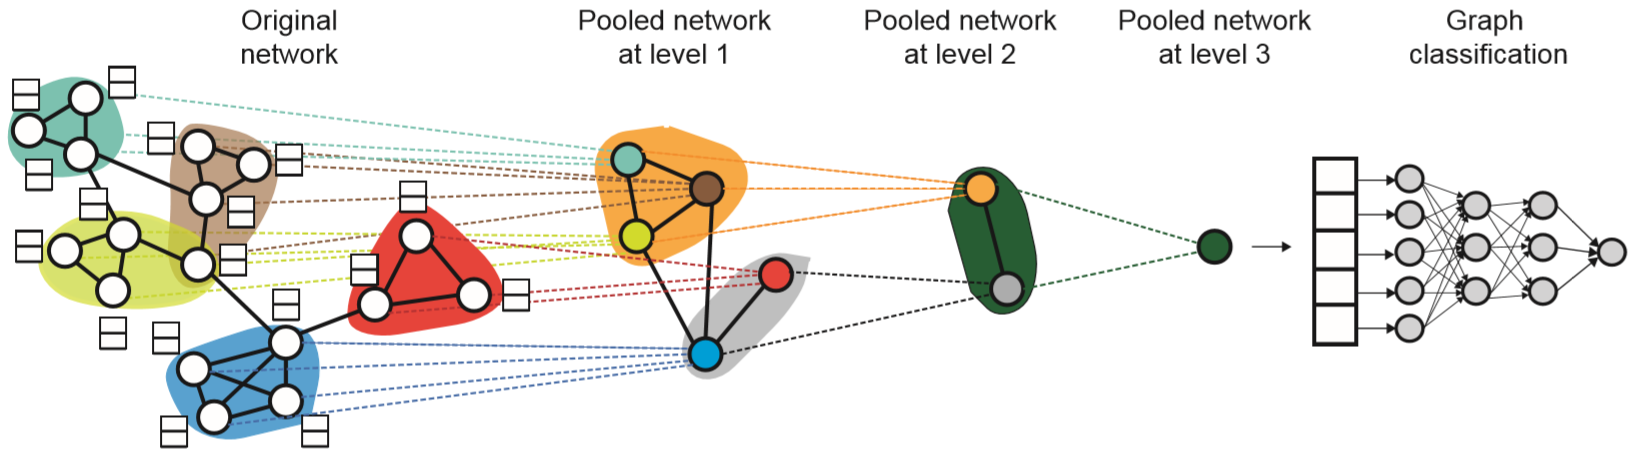
\includegraphics[width=.8\textwidth]{pics/DIFFPOOL.PNG}
	\caption{Overview of DIFFPOOL}
	\label{fig:diffpool}
\end{figure}

\paragraph{DIFFPOOL思路}DIFFPOOL的过程如Fig.\ref{fig:diffpool}所示。通过逐步将图中的结点压缩成一个节点,形成新的图的方法,逐步得到图的多个层次化的表示,最终图将被压缩成一个结点,再将这个结点的表征输入MLP中对图进行分类。为了得到图的结点表征和对图中结点进行软聚类,DIFFPOOL中一共用到了两个GNN,$GNN_{embed}$用于学习图的结点表征,$GNN_{pool}$用于学习软分配矩阵。其中的软分配矩阵的作用就是用于把$GNN_{embed}$的结点表征矩阵压缩成结点更少的图,并把邻接矩阵压缩成对应的图的连接方式。现有图$G = (X, A)$,DIFFPOOL的过程形式化表示为:
$$
Z^{(l)} = GNN^{(l)}_{embed}(A^{(l)}, X^{(l)} )
$$
$$
S^{(l)} = softmax( GNN^{(l)}_{pool}(A^{(l)}, X^{(l)} ) )
$$
$$
X^{(l+1)} = S^{(l)}Z^{(l)}
$$
$$
A^{(l+1)} = S^{(l)^\mathrm{T}} A^{(l)} S^{(l)}
$$
上式中,$l$表示GNN的第$l$层。在实际训练DIFFPOOL的过程中,论文中不仅使用了图分类作为学习的目标,同时使用了连接预测来监督模型的学习,为的是尽量使有边连接的结点被池化到同一个超点中。


\paragraph{方法解决的问题/优势}
\begin{itemize}
	\item 提出了一种新的图池化方法,使得处于类似簇/社群中的结点被压缩成一个超点
	\item 能够学习到层次化的图表征
	\item 能间接得到图的社群结构

\end{itemize}

\paragraph{方法的局限性/未来方向}
\begin{itemize}
	\item 使用其他的池化方法,减小计算代价
	\item 不太理解其中$A^{(l+1)} = S^{(l)^\mathrm{T}} A^{(l)} S^{(l)}$的原因
	\item 因为结点表征和邻接矩阵使分开来池化的,这样能保证\tred{结点表征和邻接矩阵的匹配吗}

\end{itemize}


